\chapter{Background}
\label{ch:background}

% ============================================================
% LAB GUIDE — Background (Ch.) gives the conceptual foundations a reader
% needs to follow Chapter~\ref{ch:methods}: large language models,
% how their behavior is shaped, how speech is handled in
% human--robot dialogue, and the trade-offs between locally hosted
% and cloud-hosted model deployment.
% Aim for short, intuitive coverage rather than a textbook walk-through.
% ============================================================

% TODO (compression pass before submission): the sections below currently
% read as a textbook walk-through carried over from earlier drafts.
% Trim aggressively --- target roughly two pages in total, just enough so a
% reader from outside NLP can follow Chapter~\ref{ch:methods}. Keep the
% figures and the high-level intuitions; drop the step-by-step derivations
% and push deeper detail into the inline citations.

This chapter gives a short overview of the concepts that the rest of the thesis builds on: how large language models work and how their behavior is shaped, how speech is handled in human--robot dialogue, and the trade-offs between locally hosted and cloud-hosted model deployment.
The aim is not a complete treatment but enough conceptual grounding for the design choices in Chapter~\ref{ch:methods}.


\section{Large Language Models}
\label{sec:llm_foundations}

Large Language Models (LLMs) are neural networks trained on large text corpora to predict the next token in a sequence.
Formally, an LLM estimates the conditional probability distribution
\[
P(w_t \mid w_1, w_2, \dots, w_{t-1}),
\]
the probability of the next token given all previously observed tokens.

Modern LLMs are based on the Transformer architecture~\cite{vaswani2017attention}, which replaces recurrent computation with self-attention.

\subsection*{Tokenization and Representation}

Before text can be processed by a model, it must be converted into discrete units called \emph{tokens}.
Tokens are not necessarily whole words; they may correspond to subword fragments, characters, or punctuation.

\begin{figure}[H]
    \centering
    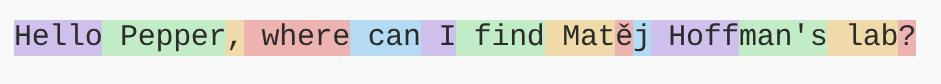
\includegraphics[width=0.85\textwidth]{src/figures/tokens.jpg}
    \caption{Example tokenization produced by the OpenAI Tokenizer tool~\cite{openai_tokenizer}.}
    \label{fig:openai_tokenizer_tokens}
\end{figure}

Each token is mapped to a high-dimensional continuous vector representation called an \emph{embedding}.
These embeddings capture semantic similarity: tokens appearing in similar contexts obtain nearby representations in vector space.

\subsection*{Autoregressive Generation}

LLMs operate autoregressively. Given an input prompt (e.g., a user query), the model generates output one token at a time.
At each step, it computes a probability distribution over the vocabulary and samples or selects the next token.
This token is appended to the sequence and becomes part of the context for the next prediction.

Complex behaviors such as summarization, dialogue, or planning emerge from this objective at scale~\cite{wei2022emergent}.

\subsection*{Context Window}

The \emph{context window} defines the maximum number of tokens the model can process at once.
All dialogue history, system instructions, retrieved documents, and intermediate tool outputs must fit within this window.
If the limit is exceeded, older tokens must be truncated or summarized.

Context limitations directly affect system design in long-running interactions and motivate external memory mechanisms such as retrieval augmentation~\cite{lewis2020rag}.

\subsection*{Practical Limitations}

Despite their capabilities, LLMs exhibit several well-known limitations:

\begin{itemize}
    \item \textbf{Hallucinations:} The model may generate fluent but factually incorrect information when the prompt lacks grounding~\cite{ji2023survey}.
    \item \textbf{Non-determinism:} Due to probabilistic sampling and internal stochasticity, outputs may vary across runs.
    \item \textbf{Limited world state awareness:} The model does not have real-time knowledge unless external information is explicitly provided.
    \item \textbf{Latency and computational cost:} Token-by-token generation introduces delay, which becomes significant in real-time robotic interaction.
\end{itemize}

\section{Adapting LLMs: Prompting, Tools, and Retrieval}
\label{sec:llm_control}

Out of the box, an LLM produces free-form text and does not automatically stay within a task definition or ground its answers in external information.
Four complementary strategies address this: fine-tuning, prompt engineering, tool calling, and retrieval-augmented generation.

\subsection{Fine-Tuning}

Fine-tuning adapts a pre-trained language model by updating its weights on additional task-specific data.
Instead of training from scratch, a base model is further optimized on curated instruction datasets, dialogue transcripts, or domain-specific data.
This approach enables specialization of tone, behavior, and knowledge distribution.

Instruction tuning and reinforcement learning from human feedback (RLHF) have been widely used to align models with desired conversational norms and safety constraints~\cite{ouyang2022training, chung2022scaling}.
Fine-tuning can significantly improve task performance and reduce undesirable behaviors in well-defined domains.

However, fine-tuning introduces important tradeoffs:

\begin{itemize}
    \item \textbf{Data demand:} A substantial amount of high-quality, task-relevant data is required.
    \item \textbf{Cost:} Training large models requires substantial compute resources.
    \item \textbf{Maintenance:} Updates to institutional knowledge require repeated retraining.
    \item \textbf{Reproducibility:} Stochastic training processes and proprietary base models complicate exact replication.
\end{itemize}

In domains where institutional knowledge changes frequently (e.g., room assignments, contact information, schedules), embedding such volatile data directly into model weights is inefficient and hard to maintain.
Systems in such domains typically rely on prompting and external tools for behavioral control and knowledge access rather than on fine-tuning.

\subsection{Prompt Engineering}

Prompt engineering refers to the structured design of input instructions that guide model behavior without modifying its internal parameters.
Modern LLMs respond strongly to in-context examples and to reasoning demonstrations provided in the prompt~\cite{brown2020language, wei2022chain}.

System-level instructions can define persona, tone, safety rules, and output structure.
Few-shot prompting provides task demonstrations that bias the model toward desired patterns of reasoning or formatting.
Output constraints (e.g., JSON schemas) further restrict generation space and improve downstream reliability.

Prompt-based control has several advantages:

\begin{itemize}
    \item No additional training cost.
    \item Immediate iteration and deployment.
    \item Separation between base model and application logic.
\end{itemize}

However, prompting does not inject new factual knowledge into the model.
It can steer style and reasoning patterns, but it cannot reliably compensate for missing or outdated information.
This limitation motivates the integration of external knowledge sources.

\subsection{Tool Calling}
\label{sec:tool_calling}

\begin{wrapfigure}{r}{0.42\textwidth}
    \vspace{-0.5\baselineskip}
    \centering
    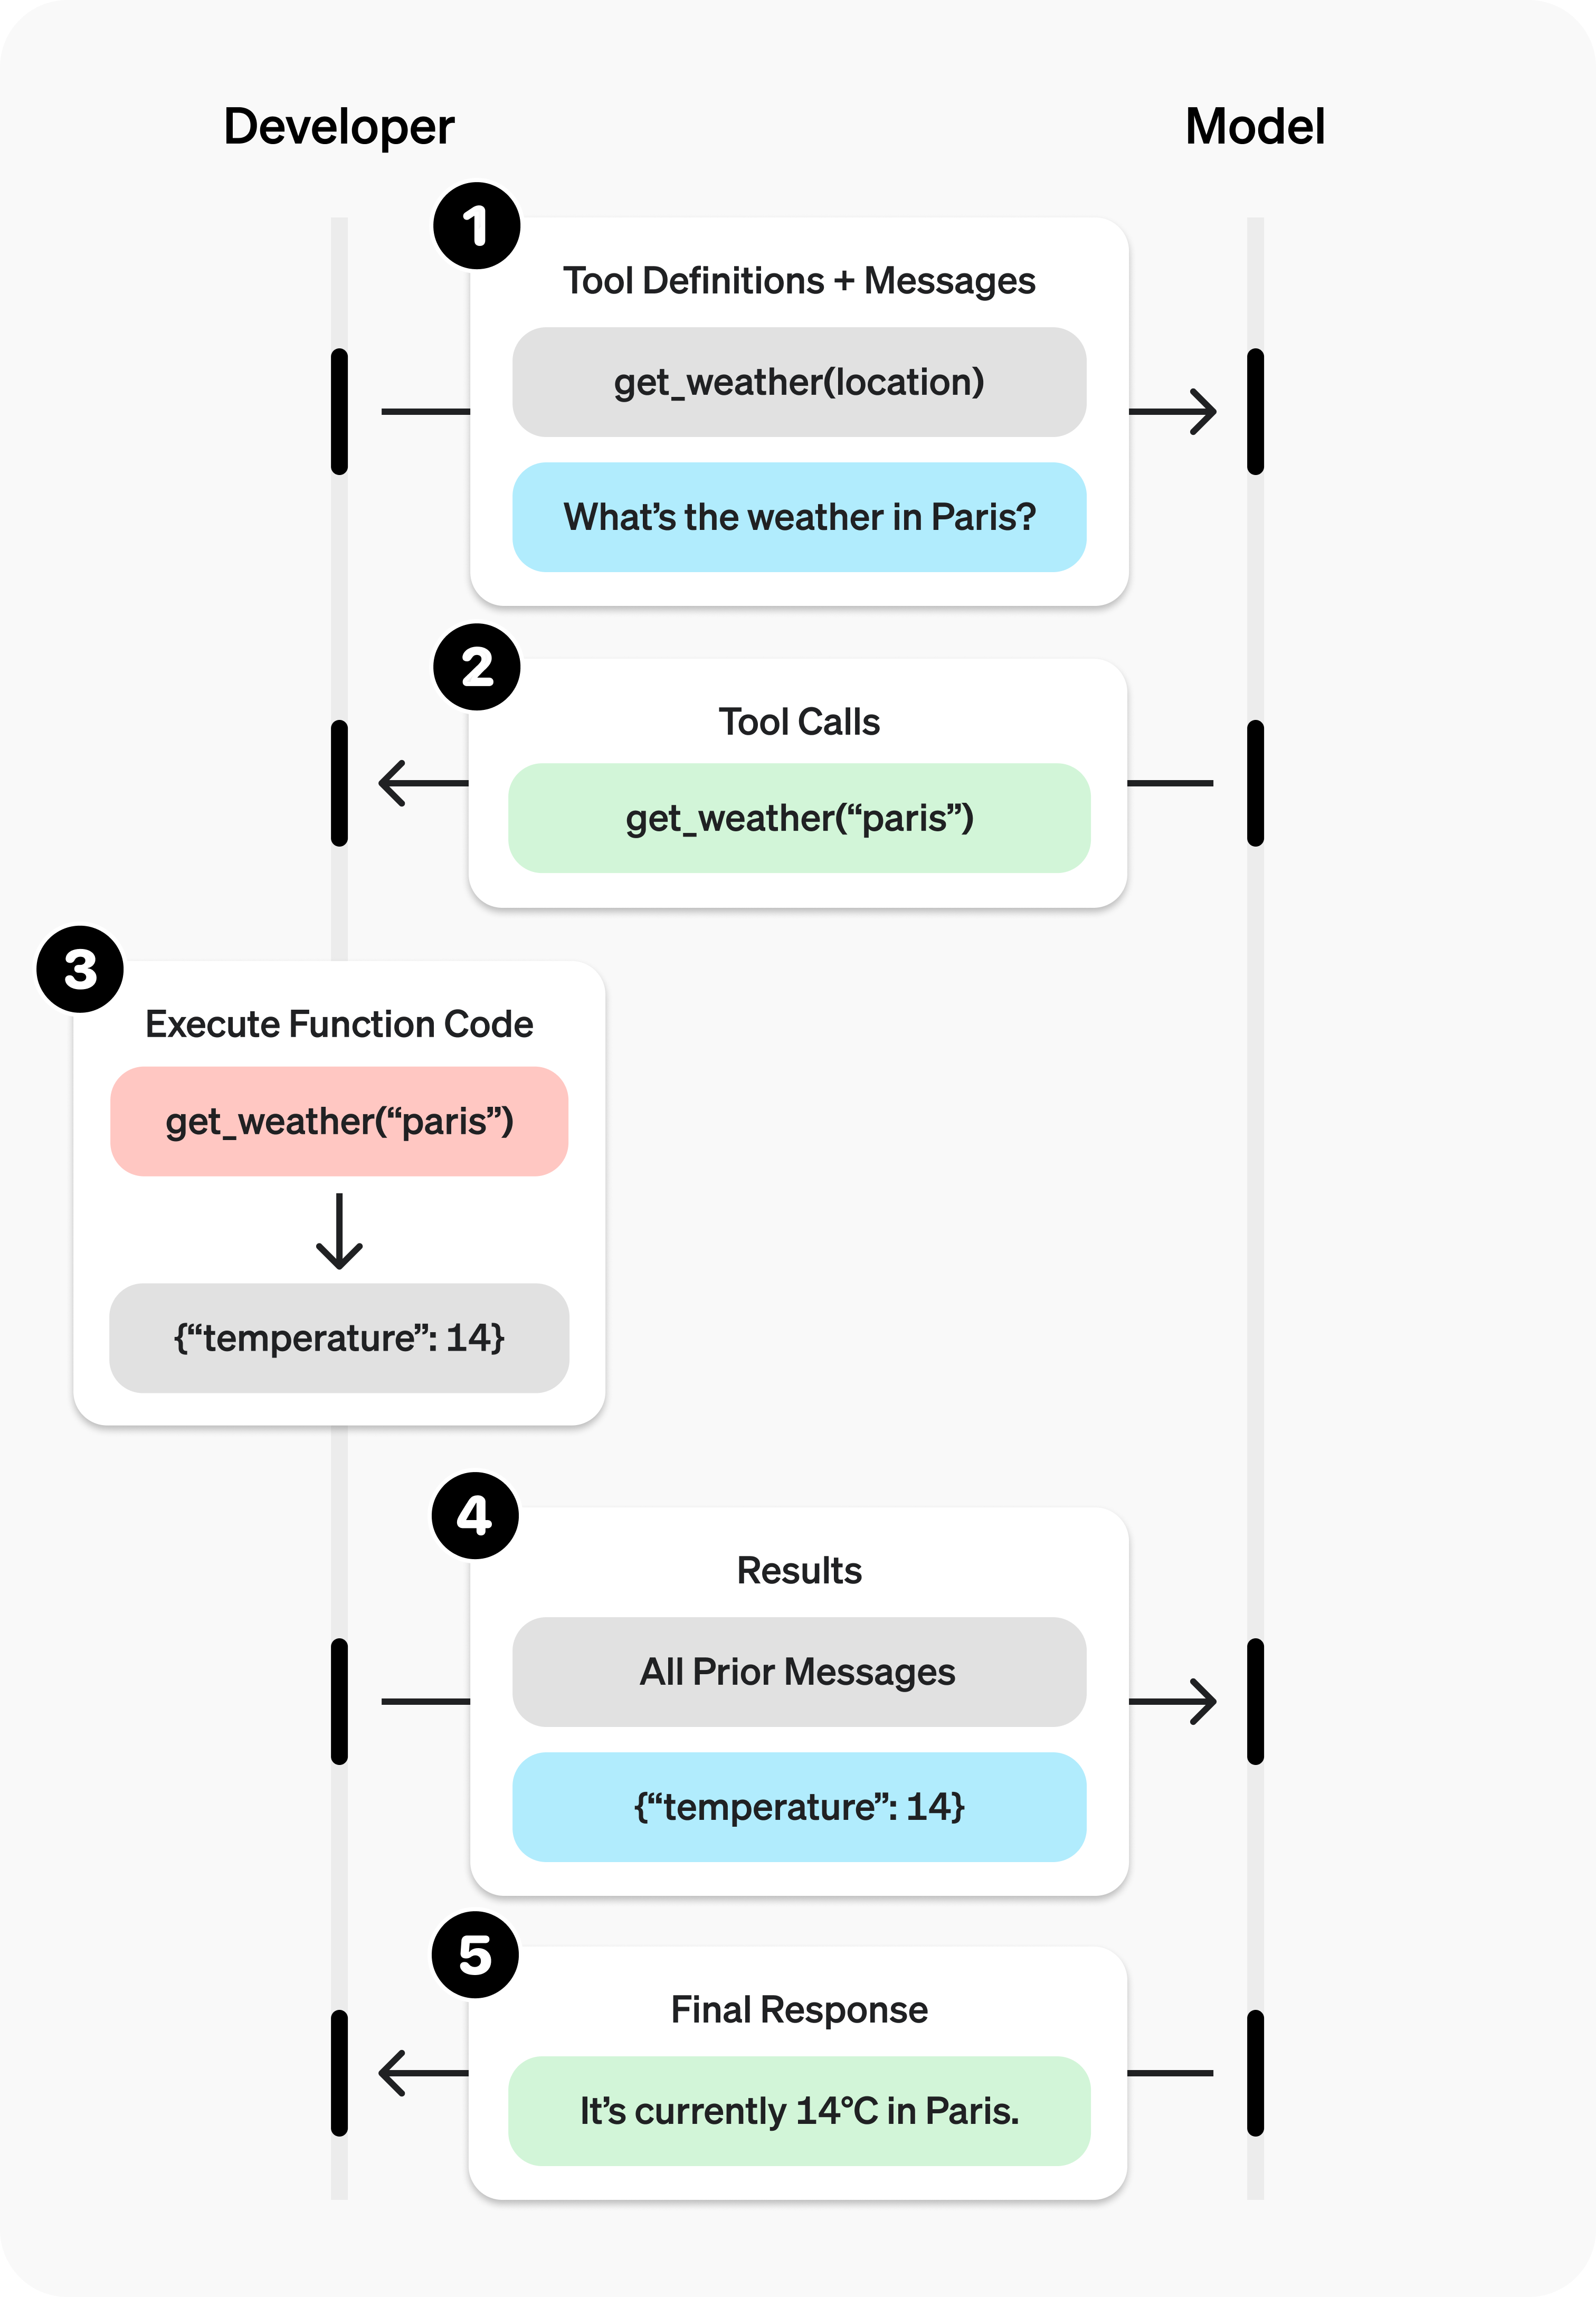
\includegraphics[width=0.40\textwidth]{src/figures/tool_calling_flow.png}
    \caption{Typical interaction loop of an LLM tool call. Source: OpenAI Function Calling Guide~\cite{openai_function_calling}.}
    \label{fig:tool_calling_flow}
\end{wrapfigure}
Tool calling (also referred to as function calling) enables an LLM to produce structured outputs that trigger executable actions instead of free-form text~\cite{schick2023toolformer, yao2023react, openai_function_calling}.
Rather than generating only natural language, the model may return a structured function call with validated arguments that correspond to a predefined interface, as formalized in modern LLM APIs~\cite{openai_function_calling}.

This mechanism separates reasoning from execution.
The LLM decides \emph{what} should be done, while external deterministic code performs \emph{how} it is done.
This is critical in embodied systems, where actions must be reliable, safe, and constrained.

Figure~\ref{fig:tool_calling_flow} illustrates the typical interaction loop, and the process consists of the following steps:


\begin{enumerate}
    \item The developer defines available tools (e.g., \texttt{get\_weather(location)}) and provides them to the model together with the user message.
    \item The model decides that answering requires structured data and produces a tool call instead of a textual reply.
    \item The application executes the corresponding function in deterministic code and obtains a result.
    \item The result is appended to the conversation context.
    \item The model generates the final user-facing response grounded in the returned data.
\end{enumerate}

This structured interaction reduces hallucinations because factual information is retrieved from verified sources rather than generated from internal model memory.

Tool implementations in embodied systems typically fall into two categories: knowledge-retrieval tools that query external sources (documents, contacts, schedules), and robot-control tools that trigger physical actions (navigation, gestures, gaze).
Both share the same structured calling mechanism, which simplifies orchestration and ensures that all external effects are mediated through validated interfaces.


\subsection{Retrieval-Augmented Generation (RAG)}
\label{sec:rag}

A baseline approach to grounding an LLM in domain-specific knowledge is to insert all relevant
documents directly into the context window. However, this strategy does not scale due to:
\begin{itemize}
    \item Context window limits,
    \item Increased token cost,
    \item Noisy or irrelevant information degrading output quality.
\end{itemize}

Retrieval-Augmented Generation (RAG) addresses this limitation by separating storage from reasoning~\cite{lewis2020rag}.
The typical pipeline consists of:

\begin{enumerate}
    \item Encoding documents into vector embeddings,
    \item Indexing them in a vector database,
    \item Retrieving semantically relevant chunks at query time,
    \item Conditioning the LLM response on the retrieved context.
\end{enumerate}

Instead of permanently embedding knowledge into model weights, RAG dynamically injects only the most relevant information into the prompt.
This improves factual grounding and reduces hallucination risk.

A common implementation pattern in embodied systems exposes retrieval as a tool call triggered during dialogue, sharing the same structured interface as robot-control tools.
This creates a unified orchestration layer in which language reasoning, information grounding, and physical action share a common mechanism.


\section{Speech Interfaces for Human--Robot Interaction}
\label{sec:multimodal_voice}

A spoken-dialogue system must process audio input, perform language reasoning, and generate speech output in real time.
Two architectures are used in practice: the modular cascaded pipeline and the integrated end-to-end audio model.

\subsection{Modular Cascaded Speech Architecture}

The modular cascaded speech architecture decomposes spoken interaction into three sequential stages:
Speech-to-Text (STT), language reasoning using a Large Language Model (LLM) and Text-to-Speech (TTS) synthesis.

In this pipeline, user speech is first transcribed into text by the STT module.
The textual transcript is then processed by the LLM, which performs dialogue reasoning and may invoke tool calls.
Finally, the generated textual response is synthesized into audio by the TTS system and played back to the user.

This architectural separation provides several advantages:

\begin{itemize}
    \item \textbf{Modularity:} Each component can be independently developed, replaced, or optimized.
    \item \textbf{Transparency:} The intermediate textual representation enables logging, inspection, and debugging.
    \end{itemize}

However, the cascaded design also introduces limitations:

\begin{itemize}
    \item \textbf{Cumulative latency:} Delays from STT, LLM generation, and TTS synthesis accumulate sequentially.
    \item \textbf{Error propagation:} Transcription errors in STT directly affect downstream reasoning.
    \item \textbf{Pipeline orchestration complexity:} Real-time coordination between independent modules requires additional engineering effort.
\end{itemize}

\subsection{Integrated End-to-End Audio Architecture}

Integrated end-to-end audio architectures model speech perception, language reasoning, and speech generation within a unified multimodal framework.
Recent multimodal foundation models operate directly on audio representations, enabling speech-in to speech-out interaction without mandatory intermediate textual stages.

Key characteristics include:

\begin{itemize}
    \item Unified perception and generation,
    \item Reduced explicit pipeline orchestration,
    \item Potentially lower end-to-end latency,
    \item Native multimodal reasoning capabilities.
\end{itemize}

The absence of an intermediate textual representation reduces transparency and complicates debugging.


\section{LLM Deployment: Local vs Cloud}
\label{sec:local_vs_cloud}

Large language models and multimodal foundation models can be deployed either locally on dedicated hardware or accessed through cloud-based APIs.
The two options differ in cost structure, performance, scalability, and data governance.

\subsection{Local Deployment}

Local deployment involves running models on privately controlled hardware, typically GPU-equipped servers.
Inference performance depends directly on available computational resources, including GPU memory capacity, compute throughput, and storage bandwidth.
Larger models generally provide improved reasoning quality and robustness, but require substantially more memory and computational power.

The primary characteristics of local deployment include:

\begin{itemize}
    \item \textbf{Hardware dependency:} Model size is constrained by available GPU memory and compute capability.
    \item \textbf{Performance--quality trade-off:} Smaller models enable lower latency and reduced resource consumption, while larger models often provide higher response quality at increased computational cost.
    \item \textbf{Fixed infrastructure cost:} After hardware acquisition, inference does not incur per-token or per-request fees.
    \item \textbf{Data sovereignty:} All data processing occurs within controlled infrastructure, reducing exposure of sensitive information.
\end{itemize}

Local deployment is particularly attractive in scenarios involving sensitive data, strict privacy requirements, or predictable high interaction volume.
However, it requires maintenance of hardware infrastructure, model updates, and system optimization.

\subsection{Cloud-Based Deployment}

Cloud-based deployment provides access to large-scale foundation models through remote APIs.
The provider manages infrastructure, scaling, optimization, and model updates.

Key properties include:

\begin{itemize}
    \item \textbf{Elastic scalability:} Compute resources scale automatically based on demand.
    \item \textbf{Access to frontier-scale models:} Very large models may be accessible without requiring local hardware.
    \item \textbf{Usage-based pricing:} Costs are typically proportional to the number of processed tokens or requests.
    \item \textbf{Reduced operational overhead:} Infrastructure management and optimization are handled by the provider.
\end{itemize}

Recurring token-based pricing can become significant under high interaction volume.
Data must also be transmitted to external servers, which may raise privacy or regulatory concerns depending on the application domain.
